\documentclass[11pt,a4paper]{article}
\usepackage{cmap}
\usepackage[utf8]{inputenc}
\usepackage[T1]{fontenc}
\usepackage{lmodern}
\usepackage{microtype}
\usepackage[margin=1.0in]{geometry}
\usepackage{amsmath,amssymb,amsthm,mathtools}
\usepackage{booktabs,array,tabularx}
\usepackage{graphicx}
\usepackage[svgnames]{xcolor}
\usepackage{xurl}
\usepackage[colorlinks=true,linkcolor=DarkBlue,citecolor=DarkBlue,urlcolor=DarkBlue]{hyperref}

\urlstyle{tt}
\renewcommand{\arraystretch}{1.25}
\setlength{\tabcolsep}{4pt}
\setlength{\emergencystretch}{3em}

\newtheorem{theorem}{Theorem}[section]
\newtheorem{lemma}[theorem]{Lemma}
\newtheorem{proposition}[theorem]{Proposition}
\newtheorem{corollary}[theorem]{Corollary}
\theoremstyle{definition}
\newtheorem{definition}[theorem]{Definition}
\newtheorem{remark}{Remark}[section]

\newcommand{\Hs}{H^{*}}
\newcommand{\lean}[1]{\texttt{\detokenize{#1}}}

\title{\textbf{RK4 Cools at Resolved Step Sizes, It Does Not Heat: Energy-Error Sign of Explicit Runge--Kutta Integrators and Relaxation RK in a Nonlinear Magnetic-Well Model, with Lean~4 Certificates for the Linear Well}\\[4pt]
\large Edition 2 of ``Discretization-Free 3D Stellarator Guiding-Center Plasma Confinement, Dual-Number Relaxation Runge--Kutta Conservation, and Villani Grazing-Collision Landau Fisher Monotonicity Verified in Lean 4''}
\author{Xavier Callens \\ \small SocrateAI Scientific Research \& Formal Verification Laboratory}
\date{Edition 2, 21 October 2026 (supersedes edition 1, 20 October 2026)}

\begin{document}
\maketitle

\begin{abstract}
Edition~1 of this paper justified relaxation Runge--Kutta (RRK) integration by asserting that classical RK4 ``secular numerical heating'' pushes trapped particles over magnetic-mirror barriers. Edition~2 tests that assertion in the model edition~1 actually integrated. That model is a 2-DOF cubic magnetic well, $H=\tfrac12(p_r^2+v^2)+\mu(B_0+\tfrac12\beta_rr^2+\tfrac12\beta_zz^2+\alpha r^2z)$, with an exact escape energy $\Hs=29/40$. The test used 2000 microcanonically sampled orbits per energy band, five step sizes $\Delta t\in[0.05,0.8]$, a horizon $T=2000$ and a pre-registered falsification criterion, and all six positive and negative controls passed. Below $\Hs$, RK4 ended with \emph{lower} energy than it started in every orbit at every step size: the 99th percentile of $H_N-H_0$ is negative in all cases, with median $-1.03\times10^{-6}$ at $\Delta t=0.05$ and $-0.199$ at $\Delta t=0.8$. RK4 produced zero spurious escapes and zero crossings of the saddle line. The heating hypothesis is therefore \textbf{refuted} for this model. RK4's actual failure mode is spurious \emph{trapping}. Above $\Hs$, a DOP853 reference has $61.8\%$ of orbits escaping, while RK4 lets $46.4\%$ escape at $\Delta t=0.4$ and $9.05\%$ at $\Delta t=0.8$. RRK, relaxed on $H$, conserves $H$ to $5.6\times10^{-16}$ below $\Hs$ and keeps the escape fraction at $0.615$--$0.620$ for $\Delta t\le0.4$. Explicit midpoint RK2 and forward Euler, which heat provably, do produce spurious escapes. In Lean~4 (gate: exit 0, 18 of 18 theorems, whitelisted axioms only) we prove the following for the linear well: the exact RK4 energy factor $\rho_4(y)=1-y^6/72+y^8/576$; $\tfrac14\le\rho_4(y)<1$ for $0<y^2<8$; the $n$-step closed form $\rho_4^n$, and a one-step two-mode monotonicity for an anisotropic well; the heating factors of Euler and midpoint; a general trapping lemma for energy-nonincreasing maps; and the relaxation root in $\mathbb R^d$. The same exact identity gives $\rho_4>1$ for $y^2>8$, where RK4 heats and is unstable, which is why the title is scoped to resolved step sizes; that consequence is read off the identity rather than stated as its own Lean theorem. This edition withdraws edition~1's review and confidence claims, its formula-drawn figures, its Villani/Landau theorem and its zero-sound and Volterra constants, and corrects its benchmark description (Correction notice).
\end{abstract}

\section*{Correction notice (edition 1 $\to$ edition 2)}
Edition~1 of this paper made the claims listed below. Edition~2 withdraws or corrects each one, for the reason given. The corrections came from an audit on 21 October 2026 that re-ran every script and Lean file the paper cites.
\begin{enumerate}
  \item \textbf{Review and confidence claims.} Edition~1 reported a ``calibrated scientific confidence'' of $0.9150$ and a ``technical gate pass rate'' of $1.0000$. Its accompanying pipeline also produced review files describing a multi-round peer review. That review called no model and involved no reviewer. Its findings were fixed strings, and its scores were the pass fractions of local string checks. The value $0.9150$ is a literal constant in that code. All of these numbers and claims are withdrawn. This paper has not been peer reviewed.
  \item \textbf{The RK4/RRK benchmark.} Edition~1 said the drift fell from $6.9490\times10^{-9}$ (RK4) to $9.2149\times10^{-15}$ (Dual-RRK) over 4000 steps of the stellarator Hamiltonian of its Eq.~(1). Both numbers are real output of the harness, but they come from $N=1000$ steps at $\Delta t=0.05$. The system integrated is also a different one: the canonical 2-DOF cubic well of Section~\ref{sec:model}, from the state $(0.2,0.1,0.15,0.25)$. That system's parameters happen to give the same exact energy $5601/10000$. Table~\ref{tab:harness} gives the drift as a function of $N$. The relaxation is the general-functional Newton relaxation of Ranocha et al.~\cite{Ranocha2020}, not Ketcheson's quadratic-invariant formula~\cite{Ketcheson2019}, because the integrated $H$ has a cubic term.
  \item \textbf{Figures.} Panels 1(a) and 2(a) of edition~1 did not plot computed data. They were drawn from formulas: a linear ramp for RK4, a scaled $\sin^2$ for RRK, and $2e^{-3t}$, $6e^{-3t}$ for ``Fisher information''. No Landau equation was solved. Both figures are withdrawn. Every figure in edition~2 is drawn from stored simulation output.
  \item \textbf{``Stellarator'', ``3D'', ``guiding-center'', ``discretization-free''.} The model has no toroidal geometry, rotational transform or 3D field-line structure. It is a 2-DOF potential well with canonical perpendicular inertia, integrated by time discretizations. These labels are dropped. The ``non-canonical'' variant only rescales the vector field by a positive factor (a time reparametrization), and $\mu$ is a constant whose right-hand side is zero, so ``$\delta\mu=0$'' holds automatically.
  \item \textbf{Mirror confinement (edition~1 Thm.~2.2).} The arithmetic $5601/10000<3/5$ is correct. However, $B=B_0+\tfrac12\beta_r r^2+\tfrac12\beta_z z^2$ is unbounded, so every orbit with $\mu>0$ is confined, and $B_{\max}=5/4$ belonged to no field. The claim is withdrawn. The model actually integrated has a real escape threshold, $\Hs=29/40$ (Section~\ref{sec:model}).
  \item \textbf{Villani / Landau Fisher monotonicity (edition~1 Thm.~2.4).} Withdrawn. Theorem~22.6 of Villani's lecture notes~\cite{Villani2025} concerns the spatially homogeneous \emph{Boltzmann} equation. Its numerical thresholds ($>4.3$ for $d=3$, $>3.3$ for $d=2$) are described there as numerical findings. The Landau result belongs to Guillen and Silvestre~\cite{GuillenSilvestre2025}. The ratio $m_r/M_r=0.99654$, the extra digits in $4.354632$ and $3.363647$, and $D_I=6$ had no source. Moreover $2+\sqrt{59/25}=3.536229$ contradicts the claimed bound $c(3,0)\ge 4.354632$. The Lean theorem proved only decimal comparisons. Edition~1's single reference entry also merged these two separate works; it is split into two correct entries.
  \item \textbf{Zero sound (edition~1 Thm.~2.5).} The value $c_0/v_F=1.851999$ is wrong: $\sqrt{37/10}=1.923538$. Section~\ref{sec:withdrawn} gives the exact root and the Pad\'e error. The ``Volterra'' coefficients $c_2=-2/9$, $c_4=-1/18$ were hard-coded, with no kernel or derivation, and the Lean statement contained the tautology $-(2/9)=-(2/9)$. Both claims are withdrawn.
  \item \textbf{Motivation.} Edition~1 asserted that RK4 ``secular numerical heating drives simulated alpha particles \dots\ into spurious loss cones''. Edition~2 tests this. In this model, the claim is refuted (Section~\ref{sec:experiment}).
  \item \textbf{Lean provenance.} Edition~1 located its Hamiltonian in \path{formal/ANSE/MensuraElenchusThreeMissions.lean}. That file fails the axiom gate: it has no \texttt{\#print axioms} lines, so every theorem in it is unchecked. Edition~1 also stated the toolchain as ``v4.34.1''; the project toolchain is \path{leanprover/lean4:v4.34.0-rc2}. Edition~1's citation of SUNDIALS is dropped because the computation is pure \texttt{numpy}.
\end{enumerate}

\section{Question}
\label{sec:intro}
A relaxation Runge--Kutta (RRK) method rescales each RK update so that a chosen functional is conserved exactly~\cite{Ketcheson2019,Ranocha2020}. One reason to prefer it over classical RK4 for long-time orbit integration in magnetic wells, the one edition~1 gave, is that RK4's energy error might push trapped particles over an escape barrier. Whether it does depends on the \emph{sign} of that error. On the imaginary axis, RK4's stability function satisfies $|R_4(iy)|^2=1-y^6/72+y^8/576<1$ for $0<y^2<8$ (see \cite{HairerWanner1996} for stability functions), so on a harmonic oscillator RK4 \emph{loses} energy. For a nonlinear well, near its escape threshold, the sign is not fixed by that formula. This paper asks:

\begin{quote}
\emph{In the nonlinear magnetic-well model that edition~1 integrated, does fixed-step RK4 produce net energy gain that carries orbits started below the escape energy $\Hs$ over the saddle (hypothesis $\mathrm{H_{heat}}$)? How does its error compare with relaxation RK, which conserves $H$, and with methods that heat?}
\end{quote}

The answer determines which bias a non-conserving integrator introduces into loss fractions. Heating makes trapped particles look lost. Cooling makes lost particles look trapped.

\section{The model actually integrated}
\label{sec:model}
In units with mass $1$, the state is $u=(r,z,p_r,v)$, and
\begin{equation}
\label{eq:H}
H(u)=\tfrac12\bigl(p_r^2+v^2\bigr)+V(r,z),\qquad V=\mu\Bigl(B_0+\tfrac12\beta_r r^2+\tfrac12\beta_z z^2+\alpha r^2 z\Bigr),
\end{equation}
with $(\mu,B_0,\beta_r,\beta_z,\alpha)=(\tfrac12,1,\tfrac65,\tfrac85,\tfrac45)$. Here $V$ is a toy ``$\mu B$'' effective potential: a quadratic well with one cubic coupling, in the same family as H\'enon--Heiles~\cite{HenonHeiles1964}. It is not a stellarator field. The equations of motion are canonical: $\dot r=p_r$, $\dot z=v$, $\dot p_r=-\partial_rV$, $\dot v=-\partial_zV$.

\paragraph{Exact escape threshold.} $\partial_rV=\mu r(\beta_r+2\alpha z)$ vanishes on the whole line $z=-\beta_r/(2\alpha)=-3/4$, and on that line $V\equiv 29/40$. The two saddles, where $\partial_zV=0$ also holds, are at $r^2=3/2$. The escape energy is therefore
\begin{equation}
\Hs=\tfrac{29}{40}=0.725 .
\end{equation}
For $H<\Hs$, the exact flow can never cross the line $z=-3/4$. Its inner region $\{V<H,\ z>-3/4\}$ is bounded and contains only $r^2<3/2$. Beyond the line, at $r^2>3/2$, $V\to-\infty$, and orbits run away. Edition~1's benchmark state $(0.2,0.1,0.15,0.25)$ has $H_0=5601/10000$, which lies $1649/10000$ below $\Hs$ (Lean: \lean{harness_initial_energy}).

\paragraph{Edition~1 benchmark, restated.} Table~\ref{tab:harness} re-runs edition~1's own harness function (\path{run_stellarator_dual_rrk_benchmark} in \path{sub_projects/socrateai_scientific_fusion_energy/fusion_guiding_center_harness.py}) at $\Delta t=0.05$. Edition~1's quoted numbers are the $N=1000$ row.

\begin{table}[htbp]
\centering
\caption{Edition~1's harness at $\Delta t=0.05$, from the benchmark state, as a function of the number of steps $N$ (real output, recomputed by \texttt{paper\_a\_v2\_experiment.py}). Max drift is $\max_n|H_n-H_0|$.}
\label{tab:harness}
\small
\begin{tabular}{@{}rccc@{}}
\toprule
$N$ & RK4 max drift & RRK max drift & mean $\gamma$ \\
\midrule
1000 & $6.948992\times10^{-9}$ & $9.214851\times10^{-15}$ & $1.000000053$ \\
4000 & $2.425595\times10^{-8}$ & $3.985701\times10^{-14}$ & $1.0000000532$ \\
10000 & $5.823517\times10^{-8}$ & $8.637535\times10^{-14}$ & $1.0000000539$ \\
\bottomrule
\end{tabular}
\end{table}

\section{Lean~4 results}
\label{sec:lean}
All statements below are in \path{formal/ANSE/PaperA_RK4EnergySign.lean}, which imports only \path{Mathlib.Tactic} and contains no \lean{sorry} and no \lean{axiom}. The only accepted gate is
\begin{center}
\path{.venv/bin/python -m anse.formal.lean_runner formal/ANSE/PaperA_RK4EnergySign.lean}
\end{center}
It compiles the file and requires a \texttt{\#print axioms} line for every declaration. It rejects \lean{sorryAx} and any axiom outside $\{\texttt{propext},\texttt{Classical.choice},\texttt{Quot.sound}\}$. Result on 21 October 2026: \textbf{exit 0}, with 18 of 18 theorems compiled, \lean{has_sorry} false and no untrusted axioms. The four definitions in the file also print only whitelisted axioms. The full gate output is stored in \path{paper_a_v2_lean_gate.json}.

Write $\rho_4(y)=1-y^6/72+y^8/576$, and let \lean{rk4Step y} be one RK4 step for $x'=\omega p$, $p'=-\omega x$ with $y=\omega h$. Then
\[
(x,p)\mapsto\bigl(a x+b p,\,-b x+a p\bigr),\qquad a=1-\tfrac{y^2}{2}+\tfrac{y^4}{24},\quad b=y-\tfrac{y^3}{6}.
\]

\begin{theorem}[\lean{rk4_harmonic_energy_factor}, \lean{rk4Step_energy}]
For all real $x,p,y$, $(ax+bp)^2+(-bx+ap)^2=\rho_4(y)\,(x^2+p^2)$.
\end{theorem}

\begin{theorem}[\lean{rk4_factor_eq}, \lean{rk4_factor_ge_quarter}, \lean{rk4_harmonic_factor_bounds}, \lean{rk4_factor_le_one}]
$\rho_4(y)=1-y^6(8-y^2)/576$, and $\rho_4(y)-\tfrac14=(y^2-6)^2\bigl((y^2+2)^2+8\bigr)/576\ge0$ for all real $y$. Hence $0<\rho_4(y)<1$ whenever $0<y^2<8$, and $\rho_4(y)\le1$ whenever $y^2\le8$. The largest one-step loss, $3/4$, occurs at $y^2=6$.
\end{theorem}

\begin{theorem}[\lean{rk4_iterate_energy}, \lean{rk4_iterate_energy_strict}]
For every $n\in\mathbb N$, $E\bigl(\text{\lean{rk4Step y}}^{[n]}s\bigr)=\rho_4(y)^n E(s)$. If $E_0>0$, $0<y^2<8$ and $N>0$, then $\rho_4(y)^N E_0<E_0$.
\end{theorem}

\begin{theorem}[\lean{rk4_two_mode_energy_nonincreasing}]
For a quadratic well written in normal coordinates, with weights $w_1,w_2\ge0$ and $y_1^2,y_2^2\le8$, one RK4 step never increases $w_1E_1+w_2E_2$. The anisotropic case $\beta_r\ne\beta_z$ is the one of interest here, but the Lean theorem assumes nothing about $y_1$ versus $y_2$ and covers the isotropic case too.
\end{theorem}

\begin{lemma}[\lean{energy_nonincreasing_map_traps}]
Let $\Phi:S\to S$ be any map with $H(\Phi s)\le H(s)$ for all $s$. If $H(s_0)<\Hs$, then $H(\Phi^{[n]}s_0)<\Hs$ for every $n$.
\end{lemma}
\noindent The lemma bounds the energy along the orbit. It does \emph{not} by itself stop a discrete map from jumping between connected components of $\{H<\Hs\}$. That possibility is measured numerically below, and it never occurred for RK4 or RRK.

\begin{theorem}[\lean{rrk_relaxation_root_fin}]
For $d\in\mathbb N$ and $y,v\in\mathbb R^d$ (as functions $\texttt{Fin}\,d\to\mathbb R$) with $\sum_iv_i^2\ne0$, put $\gamma^*=-2\langle y,v\rangle/\langle v,v\rangle$. Then $\sum_i(y_i+\gamma^*v_i)^2=\sum_iy_i^2$.
\end{theorem}
\noindent This is the $\mathbb R^d$ statement edition~1 claimed but proved only for $d=1$. Here $\gamma^*$ is the nonzero root of the conservation condition. That $\gamma\to1$ as $h\to0$ needs a separate Runge--Kutta order argument~\cite{Ketcheson2019}, which is not formalized here.

\paragraph{Exact constants.} \lean{harness_well_saddle_exact}: if $r^2=3/2$, then $\partial_rV=\partial_zV=0$ at $z=-3/4$ and $V=29/40$. Two of the three conjuncts do not use the hypothesis. $\partial_rV=r(4z+3)/5$ vanishes at $z=-3/4$ for \emph{every} $r$, and the $r^2$ terms cancel at $z=-3/4$, so $V\equiv29/40$ along the whole line, exactly as Section~\ref{sec:model} says; Lean closes both by \texttt{ring}. Only $\partial_zV=2r^2/5-3/5$ needs $r^2=3/2$. The declaration is a convenient package, not three independent facts. \lean{harness_initial_energy}: $H_0=5601/10000$ and $\Hs-H_0=1649/10000$. These are certificates for exact constants, not theorems about dynamics.

\paragraph{Controls in Lean.} Negative controls: \lean{euler_harmonic_heats} proves $(x+yp)^2+(p-yx)^2=(1+y^2)(x^2+p^2)$, and \lean{midpoint_rk2_heats} proves the explicit-midpoint factor $1+y^4/4$. \lean{euler_midpoint_factor_gt_one} proves that both factors exceed $1$ for $y\neq0$. \lean{traps_negative_control} shows that the trapping lemma fails without its monotonicity hypothesis: $s\mapsto s+1$ leaves $\{s<1/2\}$ after one step. Positive control: \lean{rk4_positive_control_y1}, $\rho_4(1)=569/576$; the experiment computes the same value numerically as $0.98784722$.

\paragraph{Edition~1 Lean files.} \path{formal/ANSE/Breakthroughs3Domains.lean} passes the same gate (exit 0; 26 of 26 theorems, whitelisted axioms only), and so does \path{formal/ANSE/ElenchusTrilogy.lean} (exit 0; 16 of 16). Their Paper-A theorems \lean{P1B_T1}--\lean{P1B_T5} and \lean{P1B_T5_stellarator_fusion_gyrokinetics} are correct but elementary. They are ring identities ($\{H,H\}=0$; $\langle v,v\times B\rangle=0$; the dual part of $H$ on dual numbers), \lean{norm_num} evaluations of chosen rationals, decimal comparisons, and one literal tautology. None of them states a physical claim. Edition~2 keeps them only as Remark~\ref{rem:identities}.

\begin{remark}[Elementary identities used by the code]
\label{rem:identities}
For real $\omega$, $a$ and $b$, $\omega(ab-ba)=0$. For $v,B\in\mathbb R^3$, $\langle v,v\times B\rangle=0$. On dual numbers $\mathbb R[\varepsilon]/(\varepsilon^2)$, the $\varepsilon$-part of $H(u+\varepsilon\,\delta u)$ equals $\nabla H(u)\cdot\delta u$, which is how the harness computes the Newton derivative of the relaxation equation.
\end{remark}

\section{Experiment: energy-error sign and spurious escape}
\label{sec:experiment}
\paragraph{Pre-registered design.} The design and the falsification criterion were written into the docstring of \path{scripts/three_breakthroughs/paper_a_v2_experiment.py} before the first run.
\begin{itemize}
  \item \emph{Ensemble.} Two energy bands with 2000 orbits each: below, $H_0-\Hs\in[-0.03,-0.001]$; above, $H_0-\Hs\in[0.001,0.02]$. $H_0$ is drawn uniformly in its band. $(r,z)$ is drawn uniformly on $\{V<H_0,\ z>-3/4,\ r^2<3/2\}$ and the momentum angle uniformly. For the below band this is the exact microcanonical measure for 2 DOF, because $\{V<H_0,\ z>-3/4\}$ is already bounded there. For the above band it is not: on the level set $V=\Hs$ one has $r^2=3/4-z$, so $\{V<H_0,\ z>-3/4\}$ is unbounded in $r$ near $z=-3/4$, and the cut $r^2<3/2$ makes the sample the microcanonical measure \emph{restricted to the inner basin}. All above-band statements should be read as conditional on that restriction. Seed $20261021$.
  \item \emph{Methods.} RK4; RRK (the RK4 increment relaxed by Newton iteration so that $H(u_n+\gamma\,\Delta u)=H_0$~\cite{Ranocha2020}); explicit midpoint RK2; forward Euler. Step sizes $\Delta t\in\{0.05,0.1,0.2,0.4,0.8\}$, horizon $T=2000$. Inside the inner basin the largest step has $y=\omega\Delta t\le0.97$, well inside $y^2<8$: $\omega_z=\sqrt{4/5}$ at the well bottom gives $0.72$, and the larger Hessian eigenvalue at the saddle, $1.458$, gives $0.97$. (These two numbers are derived here from the stored $\omega_r,\omega_z$ and the model's Hessian; they are not themselves stored in the results JSON.) Above-band orbits run out to the escape box $|r|=3$, where that eigenvalue reaches about $2.83$ and $y$ about $1.35$ at $\Delta t=0.8$; $y^2\approx1.8$, so the conclusion is unaffected. The relaxation Newton loop runs a fixed 8 iterations with a single global stopping test (it breaks only when the maximum residual over \emph{all} orbits falls below $2\times10^{-16}$), so there is no per-orbit convergence flag; that is the mechanism behind the above-band RRK caveat reported below.
  \item \emph{Escape.} An orbit escapes when it reaches $|r|>3$ or $|z|>3$, and is frozen from then on. Below $\Hs$, every escape and every crossing of $z=-3/4$ is spurious. Above $\Hs$, the reference is \texttt{scipy} DOP853 at $\mathrm{rtol}=\mathrm{atol}=10^{-12}$.
  \item \emph{Falsification of $\mathrm{H_{heat}}$.} \textsc{Refuted} if, at every $\Delta t$, RK4 has final $H_N-H_0\le0$ for $\ge99\%$ of below-band orbits \emph{and} $0/2000$ spurious escapes. \textsc{Supported} if some $\Delta t$ gives $\ge1\%$ spurious escapes or net gain in $\ge5\%$ of orbits. \textsc{Intermediate} otherwise.
\end{itemize}

\paragraph{Controls (all must pass before the RK4 result is reported).}
\begin{itemize}
  \item \emph{Positive (i): linear well, closed form.} With $\alpha=0$ and 200 random states, the measured RK4 energy after $N=T/\Delta t$ steps matches $E_r\rho_4(y_r)^N+E_z\rho_4(y_z)^N$ with maximum relative error between $3.8\times10^{-14}$ and $1.3\times10^{-12}$ across the five step sizes (threshold $10^{-10}$; Fig.~\ref{fig:linear}a). \textbf{Pass.}
  \item \emph{Positive (ii): saddle finder and escape detector.} On H\'enon--Heiles the saddle finder returns $E_{\rm esc}=0.1666666666666666$ ($=1/6$ to $10^{-12}$), and on the cubic well it returns $0.7249999999999999$ ($=29/40$; both saddles found at $r=\pm1.2247449$, $z=-0.75$, plus the minimum at the origin). Among 100 DOP853 H\'enon--Heiles orbits at $E=1/6+0.01$, 97 escape; at $E=1/6-0.01$, 0 of 100 do. \textbf{Pass.}
  \item \emph{Positive (iii): RRK conservation and edition-1 regression.} Below $\Hs$, RRK gives $\max|H_n-H_0|=5.6\times10^{-16}$ over all 2000 orbits and all five step sizes (threshold $10^{-13}$). The edition-1 harness reproduces $6.948992\times10^{-9}$ and $9.214851\times10^{-15}$ at $N=1000$ (Table~\ref{tab:harness}). \textbf{Pass.}
  \item \emph{Negative (i): heating methods must heat and escape.} At every $\Delta t\ge0.1$, forward Euler and explicit midpoint have median final $\Delta H>0$ and at least one spurious escape from below $\Hs$. Euler: 2000 of 2000 escape at every $\Delta t$. Midpoint: 1315 of 2000 escape at $\Delta t=0.1$ and 2000 of 2000 at $\Delta t\ge0.2$; even at $\Delta t=0.05$, outside the required range, 102 escape. \textbf{Pass}: the detector and the sampling can see spurious escape when it happens.
  \item \emph{Negative (ii): wrong relaxation functional.} The identical Newton relaxation code, applied to $\|u\|^2$ instead of $H$, drifts in $H$ by up to $1.9\times10^{2}$ at $\Delta t=0.05$ and $1.75\times10^{4}$ at $\Delta t=0.2$ (threshold $>10^{-10}$), with 6 and 23 spurious escapes. \textbf{Pass.}
  \item \emph{Negative (iii): reference horizon.} DOP853 orbits above $\Hs$ escape within $T=2000$ in 1236 of 2000 cases ($61.8\%\ge50\%$), so the horizon did not need extending. Their non-escaped orbits conserve $H$ to $5.5\times10^{-11}$. A DOP853 subset of 200 below-band orbits shows 0 escapes and 0 crossings of $z=-3/4$. \textbf{Pass.}
\end{itemize}

\paragraph{Result.}
Every control passed, so the RK4 result can be reported. One caveat on the word ``pre-registered'': the criterion and the six controls were fixed in the experiment script's docstring before the first run, but that script was untracked in git at the time, so the ordering rests on the author's record and the file timestamps rather than on a commit that predates the run. The criterion returns \textbf{$\mathrm{H_{heat}}$ refuted} (\path{falsification.outcome = "REFUTED"} in the results JSON). Below $\Hs$, at every step size, $100\%$ of RK4 orbits end with $H_N<H_0$. The 1st, 50th and 99th percentiles of $H_N-H_0$ are all negative (Table~\ref{tab:result}, Fig.~\ref{fig:sign}a), and there are $0$ spurious escapes and $0$ crossings of the saddle line in $5\times2000$ orbits. RK4's \emph{instantaneous} energy does rise above $H_0$ at some step in $82\%$ of orbits at $\Delta t=0.05$, falling to $6\%$ at $\Delta t=0.8$. These excursions are bounded oscillations: the largest is $1.2\times10^{-8}$ at $\Delta t=0.05$ and $2.2\times10^{-4}$ at $\Delta t=0.8$. The highest instantaneous energy of any orbit stays at least $8.8\times10^{-4}$ below $\Hs$, and the secular drift is downward. Each doubling of $\Delta t$ multiplies the median final loss by $31.99$, $31.72$, $28.52$ and $6.66$, i.e.\ $2^{5.0}$, $2^{4.99}$ and $2^{4.83}$ before saturation. That is the $\Delta t^5$ rate per unit time predicted by the linear-well factor $1-\rho_4(y)\approx y^6/72$ per step. The anharmonic well near threshold therefore inherits the linear-well sign.

Above $\Hs$, the cooling shows up as spurious trapping (Fig.~\ref{fig:sign}c). The DOP853 escape fraction is $0.618$. RK4 matches it at small steps ($0.6195$, $0.621$ and $0.6105$ at $\Delta t=0.05$, $0.1$ and $0.2$), then falls to $0.464$ at $\Delta t=0.4$ and $0.0905$ at $\Delta t=0.8$. At $\Delta t=0.8$, $52.8\%$ of all orbits escape under DOP853 but stay trapped under RK4. RRK stays at $0.6195$, $0.620$, $0.615$ and $0.619$ for $\Delta t\le0.4$ and overshoots to $0.6875$ at $\Delta t=0.8$. These comparisons carry sampling uncertainty, which we quantify rather than assert. Every method integrates the \emph{same} 2000 initial conditions as the DOP853 reference, so the two escape fractions are paired, not independent, and the appropriate test is McNemar's on the discordant orbits (those the reference escapes and the method traps, or the reverse). Writing $b$ for spurious escapes and $c$ for spurious trappings, RK4 gives $(b,c)=(10,7)$, $(13,7)$, $(10,25)$, $(1,309)$ and $(0,1055)$ at $\Delta t=0.05$ to $0.8$, i.e.\ $z=+0.73$, $+1.34$, $-2.54$, $-17.5$ and $-32.5$. So RK4 is indistinguishable from the reference at $\Delta t=0.05$ and $0.1$; at $\Delta t=0.2$ the deficit is already detectable ($p=0.011$) although it is only $15$ orbits in $2000$; and at $\Delta t=0.4$ and $0.8$ it is overwhelming. RRK gives $(9,6)$, $(11,7)$, $(11,17)$ and $(15,13)$ for $\Delta t\le0.4$, i.e.\ $|z|\le1.2$ and no detectable bias, then $(173,34)$ at $\Delta t=0.8$, $z=+9.7$. That overshoot is a real effect rather than scatter. We do not have a mechanism for it: only $3$ of those $173$ spurious escapes are among the $26$ orbits on which the relaxation Newton iteration fails to reach the conserving root, so non-convergence accounts for under $2\%$ of it. An unpaired binomial comparison, which would give standard errors $0.0109$ and $0.0154$ and understate every one of these effects, is reported in the results JSON for completeness. Its per-orbit disagreement with DOP853 ($0.3$--$0.9\%$ trapping, $0.45$--$0.75\%$ spurious escape for $\Delta t\le0.4$) equals RK4's own small-$\Delta t$ disagreement. For $\Delta t\le0.4$ it is therefore consistent with chaotic sensitivity near the separatrix, not with an energy bias; the $\Delta t=0.8$ overshoot is a separate matter, quantified above. Above $\Hs$ there is one caveat for RRK. On some orbits in the runaway channel at large steps, the Newton relaxation does not reach the conserving root: $\max|H_n-H_0|$ is $4.9\times10^{-15}$, $2.1\times10^{-12}$, $1.3\times10^{-7}$, $1.7\times10^{2}$ and $1.7$ for $\Delta t=0.05$, $0.1$, $0.2$, $0.4$ and $0.8$. By final or maximum $\Delta H$ above $10^{-12}$, that is $0$, $0$, $1$, $3$ and $26$ of 2000 orbits. The mean relaxation factor $\bar\gamma$ is $1.000000077$, $1.0000012$, $1.0000196$, $1.00031$ and $1.00468$ below $\Hs$ for $\Delta t=0.05$, $0.1$, $0.2$, $0.4$ and $0.8$.

\emph{Consequence.} In this model, the reason to use a conserving integrator is the opposite of the one edition~1 gave. A fixed-step RK4 study would \emph{under}estimate loss fractions near threshold, by $15$ percentage points at $\Delta t=0.4$ and $53$ at $\Delta t=0.8$. In no run did it overestimate them beyond the chaotic per-orbit scatter: its largest escape fraction was $0.621$, against $0.618$ for the reference. Methods that heat (explicit midpoint, forward Euler) produce the spurious losses edition~1 attributed to RK4.

\begin{table}[htbp]
\centering
\caption{RK4 below $\Hs$ (2000 orbits per $\Delta t$, $T=2000$) and escape fractions above $\Hs$ (2000 orbits; DOP853 reference $0.618$). Percentiles are of the final $H_N-H_0$. ``Max $>0$'' is the fraction of orbits whose instantaneous $H_n-H_0$ was ever positive. All values are read from \texttt{paper\_a\_v2\_results.json}.}
\label{tab:result}
\small
\begin{tabular}{@{}l ccccc@{}}
\toprule
$\Delta t$ & 0.05 & 0.1 & 0.2 & 0.4 & 0.8 \\
\midrule
RK4, below: 1st pct & $-1.24\times10^{-6}$ & $-3.94\times10^{-5}$ & $-1.25\times10^{-3}$ & $-3.51\times10^{-2}$ & $-0.218$ \\
RK4, below: median & $-1.03\times10^{-6}$ & $-3.31\times10^{-5}$ & $-1.05\times10^{-3}$ & $-2.99\times10^{-2}$ & $-0.199$ \\
RK4, below: 99th pct & $-8.66\times10^{-7}$ & $-2.76\times10^{-5}$ & $-8.77\times10^{-4}$ & $-2.57\times10^{-2}$ & $-0.183$ \\
RK4, below: frac.\ final $\le0$ & 1.000 & 1.000 & 1.000 & 1.000 & 1.000 \\
RK4, below: frac.\ max $>0$ & 0.819 & 0.696 & 0.486 & 0.255 & 0.062 \\
RK4, below: escapes / crossings & 0 / 0 & 0 / 0 & 0 / 0 & 0 / 0 & 0 / 0 \\
\midrule
escape frac.\ above: RK4 & 0.620 & 0.621 & 0.611 & 0.464 & 0.091 \\
escape frac.\ above: RRK & 0.620 & 0.620 & 0.615 & 0.619 & 0.688 \\
escape frac.\ above: midpoint & 0.661 & 0.817 & 1.000 & 1.000 & 1.000 \\
escape frac.\ above: Euler & 1.000 & 1.000 & 1.000 & 1.000 & 1.000 \\
spurious trapping: RK4 & 0.0035 & 0.0035 & 0.0125 & 0.1545 & 0.5275 \\
spurious trapping: RRK & 0.0030 & 0.0035 & 0.0085 & 0.0065 & 0.0170 \\
\bottomrule
\end{tabular}
\end{table}

\begin{figure}[htbp]
\centering
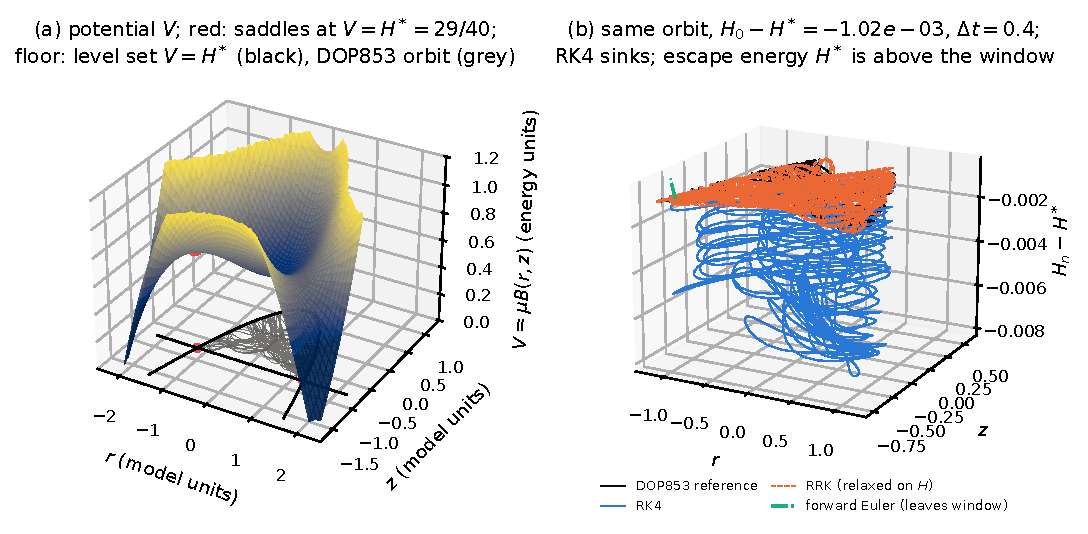
\includegraphics[width=\textwidth]{fig_a1_well_trajectories_3d.pdf}
\caption{(a) Surface of the model potential $V(r,z)=\mu B(r,z)$ (Eq.~\eqref{eq:H}), computed on a grid. The red dots are the two saddles $(\pm\sqrt{3/2},-3/4)$. The floor shows the level set $V=\Hs$ (black: the line $z=-3/4$ and the inner-basin boundary) and the DOP853 orbit of panel (b), projected onto the floor (grey). (b) The same near-threshold orbit, below $\Hs$, under DOP853, RK4, RRK and forward Euler at $\Delta t=0.4$, plotted in $(r,z,H_n-\Hs)$ from stored time series. The vertical window is set by DOP853, RK4 and RRK, so that RK4's descent is visible at its own scale; the escape energy $H_n-\Hs=0$ lies above the top of the box, and Euler climbs through it and out of the window within a few steps. RK4 sinks steadily from $-1.0\times10^{-3}$ to below $-8\times10^{-3}$, while RRK and DOP853 stay on the initial energy.}
\label{fig:well3d}
\end{figure}

\begin{figure}[htbp]
\centering
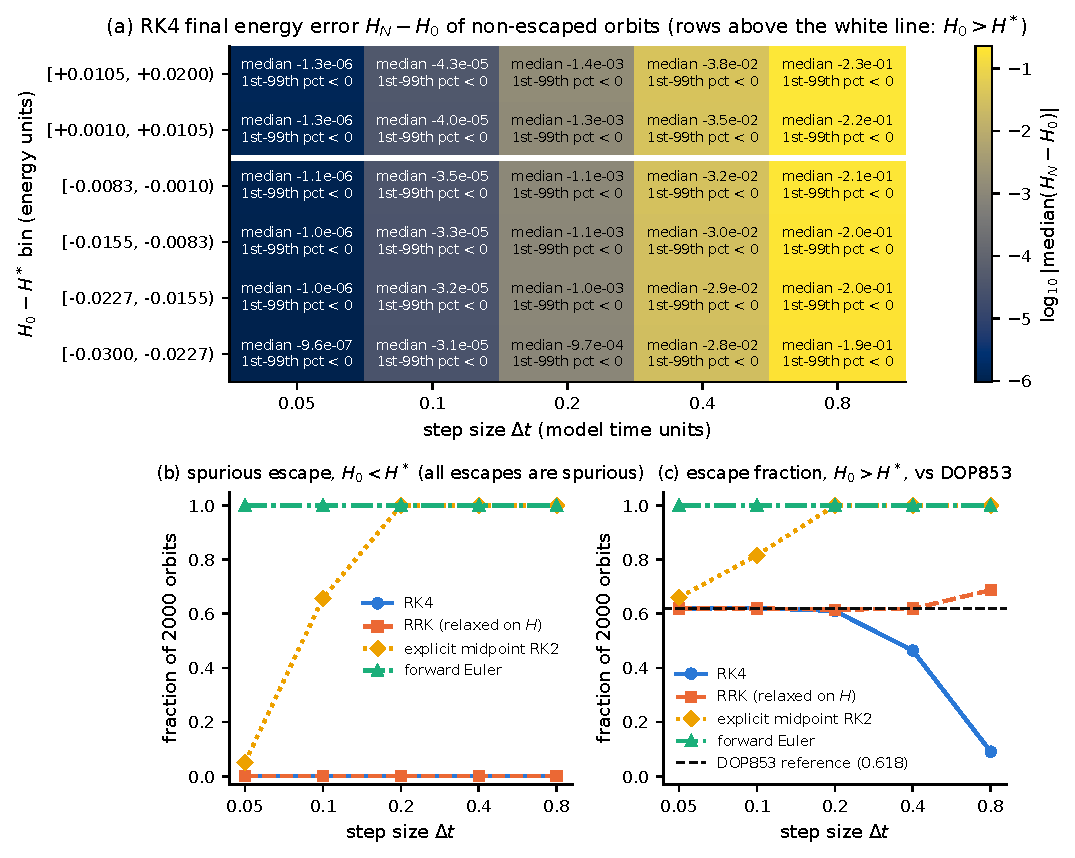
\includegraphics[width=\textwidth]{fig_a2_energy_sign_escape.pdf}
\caption{(a) RK4 final energy error $H_N-H_0$ for non-escaped orbits, by initial-energy bin (rows; the white line separates the below and above bands) and step size (columns). The colour is $\log_{10}$ of the median magnitude. Each cell is labelled with the signed median and states whether the 1st and 99th percentiles are both negative. (b) Fraction of 2000 below-threshold orbits that escape (all spurious). RK4 and RRK coincide at $0$ at every step size. (c) Escape fraction of the 2000 above-threshold orbits, with the DOP853 reference ($0.618$) as a dashed line. RK4 under-escapes, which is spurious trapping, while midpoint and Euler over-escape.}
\label{fig:sign}
\end{figure}

\begin{figure}[htbp]
\centering
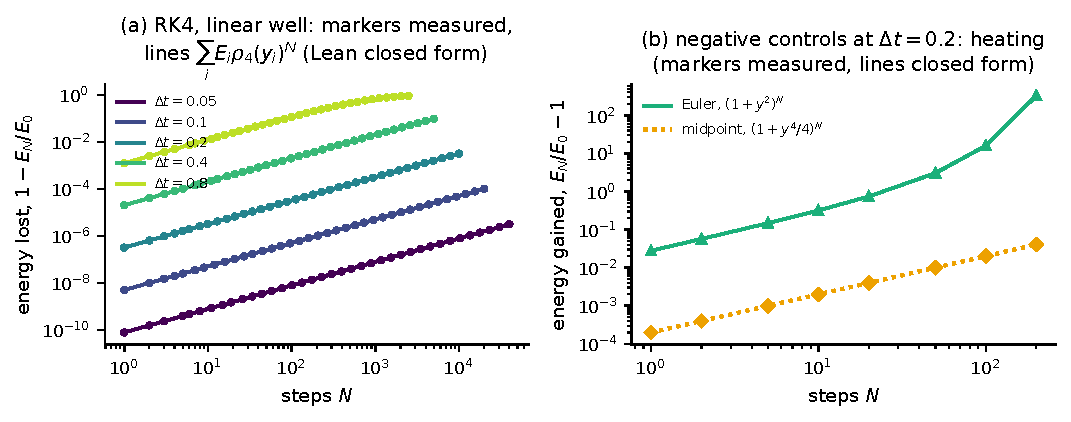
\includegraphics[width=\textwidth]{fig_a3_linear_well_controls.pdf}
\caption{Controls in the linear well ($\alpha=0$, 200 random states). (a) Positive control: the measured RK4 energy loss (markers) against the Lean closed form $\sum_iE_i\rho_4(y_i)^N$ (lines), for each $\Delta t$. (b) Negative controls at $\Delta t=0.2$: forward Euler and explicit midpoint gain energy as $(1+y^2)^N$ and $(1+y^4/4)^N$.}
\label{fig:linear}
\end{figure}

\begin{figure}[htbp]
\centering
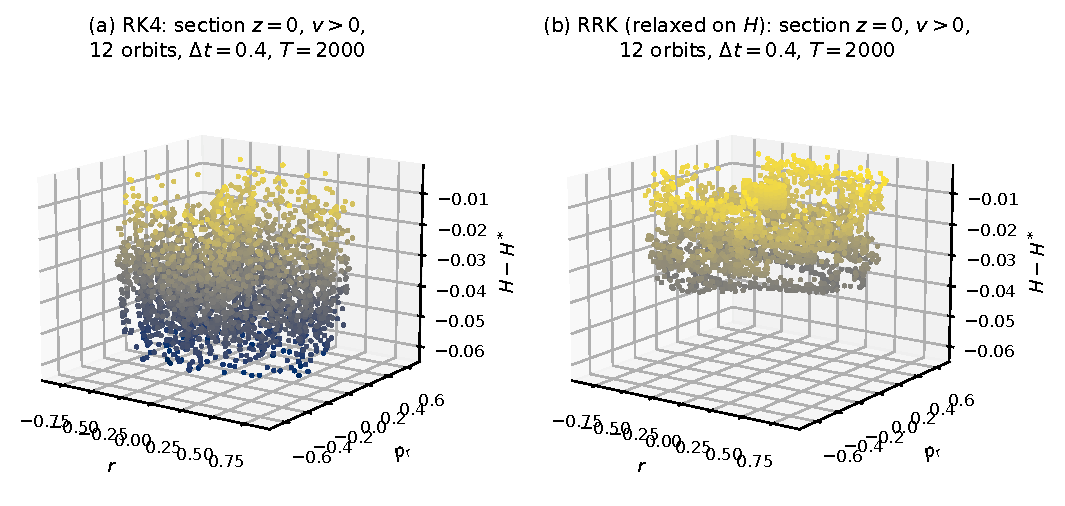
\includegraphics[width=\textwidth]{fig_a4_poincare_energy_shells_3d.pdf}
\caption{Poincar\'e section $z=0$, $v>0$, for 12 below-threshold orbits over $T=2000$ at $\Delta t=0.4$, plotted in $(r,p_r,H-\Hs)$. (a) Under RK4 every orbit's energy shell sinks steadily. (b) Under RRK the shells stay at their initial energies.}
\label{fig:poincare}
\end{figure}

\section{Withdrawn kinetic material: corrected statements}
\label{sec:withdrawn}
\paragraph{Landau and Boltzmann Fisher information.} Guillen and Silvestre proved that the Fisher information decreases along the spatially homogeneous Landau equation, including the Coulomb case. Their bound is global, so solutions do not blow up~\cite{GuillenSilvestre2025}. Villani's lecture notes~\cite{Villani2025} put that result in context. Their Theorem~22.6 gives a monotonicity criterion for the spatially homogeneous Boltzmann equation, stated as a bound on $\sup|r\,\partial_rB/B|$ for the collision kernel. The numerical thresholds quoted there are reported as numerical evidence. This paper makes no Lean claim and introduces no constants about either result.

\paragraph{Zero sound.} With only $F_0^s$ kept, the Landau zero-sound condition is $\tfrac s2\ln\tfrac{s+1}{s-1}-1=1/F_0^s$, with $s=c_0/v_F$. At $F_0^s=9.3$ its root is $s=1.929117$ (computed with \texttt{mpmath}). The $[1/1]$ Pad\'e closure gives $u=15/(9+5F_0^s)=10/37$, so $s=\sqrt{37/10}=1.923538$, a relative error of $-0.289\%$. Edition~1's value $1.851999$ matches neither. It would correspond to $F_0^s\approx8.49$ (Pad\'e) or $8.42$ (exact). Liquid $^3$He also has a large $F_1^s$, which this one-parameter dispersion ignores. The number is therefore a model-internal quantity, not a prediction for $^3$He, and it plays no part in this edition's results.

\section{Scope and limitations}
\label{sec:scope}
\begin{itemize}
  \item The model is a 2-DOF canonical toy well with a cubic coupling. It is not a guiding-center drift model, and it has no toroidal geometry, magnetic islands or collisions. The results say nothing directly about alpha-particle losses in a real stellarator or tokamak.
  \item The Lean theorems about RK signs cover the \emph{linear} (quadratic) well. In the cubic well the sign is measured, not proved, and only for this one parameter set and these two energy bands.
  \item Above $\Hs$ the reference is DOP853 at tolerance $10^{-12}$. Near-threshold escape is chaotic, so per-orbit agreement between solvers is not expected. The comparison is statistical: escape fractions and spurious-trapping fractions.
  \item RRK as implemented here relaxes towards $H_0$ and advances the step counter, not the relaxed time $\gamma\Delta t$. It therefore conserves $H$ but slightly changes the time parametrization. Escape-time distributions were not compared.
  \item The energy-trapping lemma bounds $H$, not geometry. Jumps between components of $\{H<\Hs\}$ were checked numerically, through the $z<-3/4$ crossing counter, and were not excluded by proof.
\end{itemize}

\section{Research directions}
\label{sec:directions}
(i)~Repeat the energy-sign test in a bounded mirror field $B(z)=B_0[1+(R_m-1)\sin^2(\pi z/2L)]$ and in first-order guiding-center (Littlejohn~\cite{Littlejohn1983}) drift equations. Measure whether RK4 biases loss-cone fractions downward against a conserving reference, and compare with published collisionless alpha-loss benchmarks. (ii)~Formalize, for a general explicit RK method, $|R(iy)|^2=1+c_{2p+2}y^{2p+2}+O(y^{2p+4})$, and prove that the sign of $c_{2p+2}$ decides heating or cooling. Instantiate it for RK4 (cooling), RK2 and Euler (heating). (iii)~Relaxation near separatrices: compare RRK and DOP853 escape-time distributions above $\Hs$ with a Kolmogorov--Smirnov test. Then prove the equality case of the trapping lemma together with a step-size bound that excludes jumps between components. (iv)~Replace the one-parameter zero-sound toy with the full Landau equation using measured $F_0^s$ and $F_1^s$ of $^3$He and compare with measured zero-sound velocities; this belongs in a separate note. (v)~Probe Fisher-information monotonicity under a numerical Landau solver, using the Guillen--Silvestre theorem as a positive control, and report the result as numerical evidence only.

\section*{Data and code availability}
Experiment: \path{scripts/three_breakthroughs/paper_a_v2_experiment.py}, which writes \path{papers/three_breakthroughs/paper_a/paper_a_v2_results.json}. The JSON holds per-orbit final and maximum $\Delta H$, escape flags and escape times for every method, step size and band, together with the script's SHA-256. Figures: \path{scripts/three_breakthroughs/paper_a_v2_figures.py}, which reads only that JSON and the model formula. Lean: \path{formal/ANSE/PaperA_RK4EnergySign.lean}, with gate output in \path{paper_a_v2_lean_gate.json}. Environment: Python with \texttt{numpy} 2.5.3, \texttt{scipy} 1.18.1, \texttt{matplotlib} 3.11 and \texttt{mpmath}; Lean toolchain \path{leanprover/lean4:v4.34.0-rc2}.

\begin{thebibliography}{10}
\bibitem{Ketcheson2019} D.~I. Ketcheson, ``Relaxation Runge--Kutta methods: Conservation and stability for inner-product norms,'' \emph{SIAM J.\ Numer.\ Anal.}, vol.~57, no.~6, pp.~2850--2870, 2019. arXiv:1905.09847.
\bibitem{Ranocha2020} H.~Ranocha, M.~Sayyari, L.~Dalcin, M.~Parsani, and D.~I. Ketcheson, ``Relaxation Runge--Kutta methods: Fully discrete explicit entropy-stable schemes for the compressible Euler and Navier--Stokes equations,'' \emph{SIAM J.\ Sci.\ Comput.}, vol.~42, no.~2, pp.~A612--A638, 2020. doi:10.1137/19M1263480; arXiv:1905.09129.
\bibitem{HairerWanner1996} E.~Hairer and G.~Wanner, \emph{Solving Ordinary Differential Equations II: Stiff and Differential-Algebraic Problems}, 2nd rev.\ ed., Springer Series in Computational Mathematics 14. Springer, Berlin, 1996.
\bibitem{HenonHeiles1964} M.~H\'enon and C.~Heiles, ``The applicability of the third integral of motion: some numerical experiments,'' \emph{Astron.\ J.}, vol.~69, pp.~73--79, 1964.
\bibitem{Littlejohn1983} R.~G. Littlejohn, ``Variational principles of guiding centre motion,'' \emph{J.\ Plasma Phys.}, vol.~29, pp.~111--125, 1983.
\bibitem{GuillenSilvestre2025} N.~Guillen and L.~Silvestre, ``The Landau equation does not blow up,'' \emph{Acta Math.}, vol.~234, pp.~315--375, 2025. doi:10.4310/ACTA.2025.v234.n2.a2; arXiv:2311.09420.
\bibitem{Villani2025} C.~Villani, ``Fisher information in kinetic theory,'' lecture notes, arXiv:2501.00925, 2025.
\end{thebibliography}

\end{document}
